\section{Coordination Protocol}

We assume that the clients connecting to \textit{TravelGood} are stand-alone applications calling our web services. This process starts by sending a customer/client reference identification through the \textit{CreateItinerary} operation, which will create a unique itinerary for the client. In the interaction with the client, the state itinerary changes and this is represented in the state diagram below (see figure \ref{statediagram}).  

In the state diagram several operation that can change the state of the itinerary are defined. Most of them, such as \textit{AddToItinerary}, \textit{GetHotels/Flights}, \textit{BookItinerary}, \textit{CancelItinerary} are self explanatory and well-defined in the project description. However, we should mention that \textit{TerminateItinerary}, although possible from all states (unbooked, booked, cancelled) has different meanings. The user is able to terminate the itinerary by calling the \textit{CancelItinerary} operation in the unbooked state. Concurrently, in the booked and cancelled states, it might happen that the itinerary is terminated whenever the date of a flight or a hotel has passed. 

As soon as an itinerary is terminated, it is removed from \textit{TravelGood}'s record therefore its status can not be called for anymore. 


\begin{figure}[H]
\centering
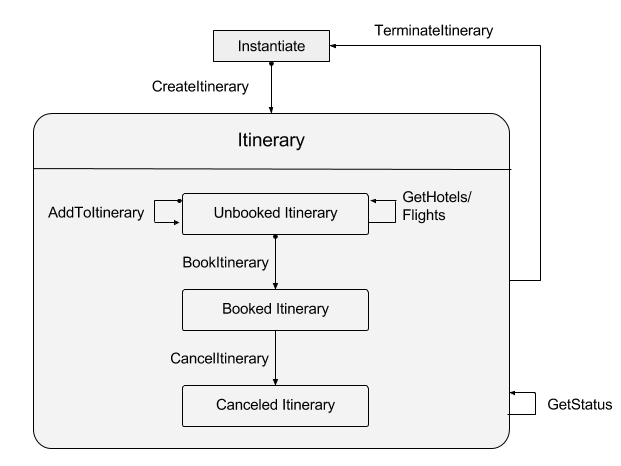
\includegraphics[width=0.6\textwidth]{images/StateDiagram}
\caption{State Diagram for the coordination protocol between the client and \textit{TravelGood}.}
\label{statediagram}
\end{figure}

The coordination process between \textit{TravelGood}, \textit{LameDuck} and \textit{NiceView} are similar for both our REST and BPEL implementations. Communication with the client happens only via the \textit{TravelGood} web service which will afterwards concurrently connect to the external web services (\textit{LameDuck} and \textit{NiceView}). Moreover, both \textit{LameDuck} and \textit{NiceView} call operations from the \textit{FastMoney} web service. All the connections between client the and services are portrayed in figure \ref{sequencediagram}. 

\begin{figure}[H]
\centering
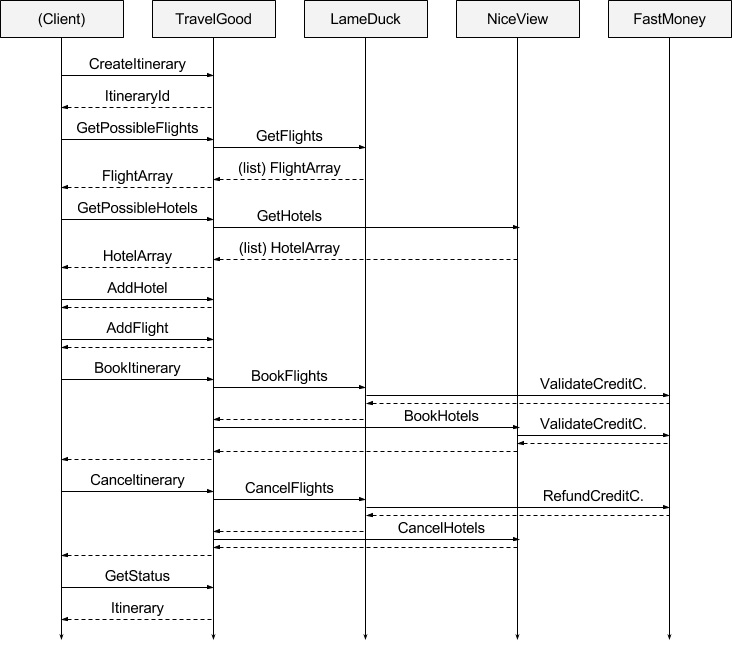
\includegraphics[width=0.6\textwidth]{images/SequenceDiagram}
\caption{Sequence Diagram for TravelGood, LameDuck and NiceView.}
\label{sequencediagram}
\end{figure}

As it can be seen as mentioned above, the client only interacts with the \textit{TravelGood} service which will afterwards start a new itinerary and return its identifier. In BPEL, \textit{TravelGood} creates a GUID identification for further communication whereas in REST, a unique string identifier is used. After the itinerary has been created, the client can request available flights and hotels from \textit{TravelGood}, which will in turn request the info from the \textit{LameDuck} and \textit{NiceView} services. The result of \textit{GetFlights} and \textit{GetHotels} operations will be an itinerary which holds two arrays, one for the list of flights and one for the list of hotels. 

During the booking (\textit{BookItinerary}) process, the client application is required to also send the bank information along with the itinerary id. This operation can return a fault if booking fails and all exceptions are handled properly (see \ref{webserviceimplementations}. Web Service Implementations). 
Similarly, the cancel itinerary operation (\textit{CancelItinerary}) also requires a booking number and credit card info and can return an error if some parts of the cancellation fail.
